\documentclass[a4paper,11pt]{article}
\usepackage[utf8]{inputenc}
\usepackage{algorithmic}
\usepackage{algorithm}
\usepackage{pst-plot}
\usepackage{graphicx}
\usepackage{endnotes}
\usepackage{graphics}
\usepackage{floatflt}
\usepackage{wrapfig}
\usepackage{amsfonts}
\usepackage{amsmath}
\usepackage{verbatim}
\usepackage{hyperref}
\usepackage{multirow}
\usepackage{pdflscape}
\usepackage{enumitem}
\usepackage[normalem]{ulem}

\usepackage{hyperref}
\hypersetup{pdfborder={0 0 0 0}}

\pdfpagewidth 210mm
\pdfpageheight 297mm 
\setlength\topmargin{0mm}
\setlength\headheight{0mm}
\setlength\headsep{0mm}
\setlength\textheight{250mm}	
\setlength\textwidth{159.2mm}
\setlength\oddsidemargin{0mm}
\setlength\evensidemargin{0mm}
\setlength\parindent{7mm}
\setlength\parskip{0mm}

\newenvironment{exercise}[3]{\paragraph{Exercise #1: #2 (#3pt)}\ \\}{
\medskip}
\newcommand{\question}[2]{\setlength\parindent{0mm}\ \\$\mathbf{Q_#1:}$ #2\ \\}

\author{\large{Tambet Matiisen, Raul Vicente}}
\title{\huge{Introduction to Computational Neuroscience}\\\LARGE{Practice on Artificial Neural Networks}}

\begin{document}
\maketitle

\textbf{A request:} Please track how long it will take to complete this set of exercises. Add this time to your final report.
\ \\

%
% Intro
%
In this session we are going to have a brief look on artificial neural networks. We start with simplest artificial neuron model called perceptron. Then we will see how simple feed-forward neural networks can be thought of as universal function approximators and what their limitations are. Finally we will use artificial neural network to recognize handwritten digits.

%
% Perceptron
%
\begin{exercise}{1}{Perceptron}{1}

\begin{wrapfigure}{r}{0.3\textwidth}
	\centering
	\vspace{-12pt}
	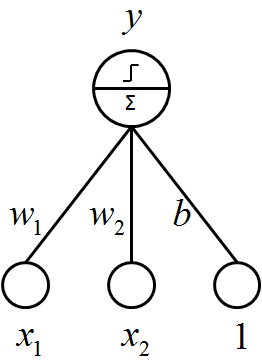
\includegraphics[width=0.22\textwidth]{perceptron.png}
	\caption{Simple perceptron}
	\label{fig:perceptronexample}
	\vspace{-5pt}
\end{wrapfigure}

Perceptron is the simplest artificial network model invented by Frank Rosenblatt in late 1950s. He added learning rule to McCulloch-Pitts neuron, that allows it to learn certain functions from example inputs and outputs.

Perceptron works on binary data – both its inputs $x_j$ and output $y$ are ones or zeros. Output 1 or 0 can be thought of as binary classification – whether object represented by input  belongs to certain class or not. 

Perceptron’s weights $w_j$ can be any real numbers. Its prediction is calculated with following formula:

$$
y = \left\{
	\begin{array}{l l}
		1, \text{if } x_1 w_1 + ... + x_m w_m + b \geq 0\\
		0, \text{otherwise}
	\end{array}
	\right.
$$

Here $b$ is the bias term, that is added to the sum. In practice it is easier to just add additional input, which is always one. Then we don’t have to treat bias as special, it is just additional weight. Learning rule for perceptron is very simple:

$$
w_j = w_j + (t_i - y_i) x_{ij}
$$

Index $i$ is used to denote $i$th data sample. Learning rule must be applied for all datasamples and for each weight. You will continue updating the weights until all data samples are classified correctly.

It turns out, that perceptron is always able to successfully learn classification rule for datasets, which are \textit{linearly separable} (data points can be separated by line in case of two intputs, plane in case of three inputs or hyperplane in case of input of any dimensionality). If the dataset is not linearly separable, perceptron will never \textit{converge} (settle to certain weight values). \newline

Example code for this exercise is in \texttt{perceptron.m}. Your task is to fill in the perceptron learning rule and decide for four example datasets if they are linearly separable or not. In your report include final image with decision boundary for all four datasets. For linearly separable datasets also add approximate number of steps to convergence.

\end{exercise}

%
% Sinusoid
%
\begin{exercise}{2}{Function Approximation}{1.5}

Artificial neural networks can be thought of as universal function approximators. Indeed, Universal Approximation Theorem states, that feed-forward network with single hidden layer containing finite number of neurons can approximate any continous function to any precision. In practice this theorem is of no use, because:
\begin{itemize}
  \item it states only, that these functions can be \uline{represented} by feed-forward network with one hidden layer, it doesn’t say anything if they are \uline{learnable};
  \item construction used in the proof uses huge number of neurons in hidden layer, which would be unreasonable for any practical application;
  \item as the theorem doesn’t consider learnability, it doesn’t state anything about how well the networks generalizes to samples outside of training data.
\end{itemize}

But it still nice result to guide your thinking – if some problem can be described as a function calculating output from several inputs, then it probably can be approximated with artificial neural network.\newline

\begin{wrapfigure}{r}{0.3\textwidth}
	\centering
	\vspace{-12pt}
	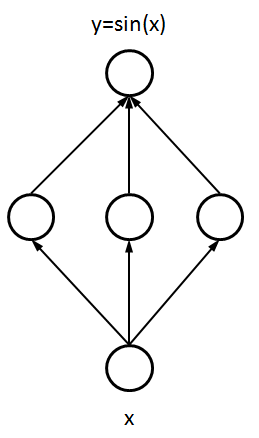
\includegraphics[width=0.20\textwidth]{sine.png}
	\label{fig:sineexample}
	\vspace{-5pt}
\end{wrapfigure}

In this practice session we are going to approximate sine function using neural network. This neural network is very simple – it consists of just one input node (the $x$), several hidden nodes and just one output node ($y = sin(x)$).

Hidden nodes use sigmoid activation function to achieve non-linearity. Output node is linear, no activation function is applied. Loss function is simple squared error:

$$
L = \frac{1}{2n}\sum_{i=1}^{n} (t_i - y_i)^2
$$

It calculates average loss over all data points in training set. \newline

For this exercise run the code in \texttt{sinusoid.m} and answer following questions:
\question{1}{Why don't we always get the same result during training? Why we sometimes achieve better approximation and sometimes worse?}
\question{2}{What is the minimum number of hidden nodes to approximate sinusoid with four bumps (like in the example given)? Include figure with your report. I’m asking for occasional (or theoretical) possibility, not that it approximates reliably with that many hidden nodes. \textbf{Bonus:} Why that might be? Function \texttt{plot\_sinusoid\_components(test\_x, nn)}  might give some hints.}
\question{3}{Apply network to inputs outside of training range, for example from $-4\pi$ to $4\pi$. How well the network generalizes to data outside of training range? Include figure.}

\end{exercise}

%
% MNIST
%
\begin{exercise}{3}{Classification of handwritten digits}{1.5pt + bonus 1}

Finally we will use artificial neural network to classify handwritten digits. For that we are going to use MNIST dataset, that was historically very important. This dataset was used to train convolutional neural networks by Yann LeCun et al. and the resulting system was one of the first commercial successes of neural networks in 1990s. At some point it was used to read 10\% of the checks in North America. It is widely used bencmark even today, because it's fast to train even on modest CPU and there is plenty of baseline performances to compare to.

Code for this excercise is in file \texttt{mnist.m}. For neural networks we are making use of DeepLearnToolbox toolkit by Rasmus Berg Palm. The tookit is already included with your download in folder \texttt{DeepLearnToolbox}. Feel free to explore the source in \texttt{DeepLearnToolbox/NN} folder, it is quite clean Matlab code.

After you have run the code and got initial results, your job is to improve classification accuracy. For that you need to tune learning rate, weight decay, number of hidden nodes and number of epochs (iterations over full data set). As tuning neural networks can be quite tedious and frustrating, here are few guidelines:

\begin{enumerate}
  \item Start with learning rate. Try 1 first and then go down by powers of ten, i.e. 1, 0.1, 0.01, 0.001 and so on. Use the first value, when the loss graph is stable (without zig-zags) and goes down. To squeeze out the last bit, you can try values between powers of ten, but usually you don't gain much.
  \item Once you have stabilized the learning, try to increase number of hidden nodes and see if testing error improves. 
  \item If your network is well tuned, then you should see overfitting, which means that network learns training examples, but doesn't generalize to the test set. You can detect this from large gap between training and validation misclassification rate. Time to bring in weight decay! Start with very small values and increase in powers of ten till test error starts to get worse, i.e. 0.00001, 0.0001, 0.001, 0.01, 0.1.
  \item Mind that there is a delicate interplay between the parameters – if you increase weight decay, then you might need to increase also learning rate; if you increase number of hidden nodes, you might need to decrease learning rate and so on.
  \item Finally, if loss function seems to have steady downward direction, increase number of epochs and see how low it goes. Usually it plateaus at some point and there is no reason to train further.
\end{enumerate}

Include figure with training and validation error in your report, along with testing error. You are expected to achieve at least 3\% test error rate. \textbf{Bonus point awarded to everybody with test error below 2\%!}

\end{exercise}



%
% Adaline video
%
\begin{exercise}{4*}{Science in Action}{bonus 1}

For this excercise you have to watch one cool video from 1960s. It's about simple analog neuron called ADALINE invented by Bernard Widrow. With all the recent hype around deep learning, it is refreshing to see how much of that was already in place in 1960s.

Watch the video here: \url{https://www.youtube.com/watch?v=IEFRtz68m-8} (until 21:43)

\question{}{What applications for adaptive neurons people foresaw already in 1960s?}

\end{exercise}


\ \\
\ \\
\ \\
\ \\
\ \\
Please submit a \texttt{pdf} report with answers to the questions and comments about your solutions. Include figures, explanations and essential pieces of code. Do not include the code itself as a separate file, your report should give good understanding of what you have done. Please mark how long it took to complete this set of exercises. Upload the \texttt{pdf} to the practice session page on the course website.

\end{document}
